%  LaTeX support: latex@mdpi.com
%  In case you need support, please attach all files that are necessary for compiling as well as the log file, and specify the details of your LaTeX setup (which operating system and LaTeX version / tools you are using).

% You need to save the "mdpi.cls" and "mdpi.bst" files into the same folder as this template file.

%=================================================================
\documentclass[journal,article,submit,moreauthors, pdftex,10pt,a4paper]{mdpi} 
%--------------------
% Class Options:
%--------------------
% journal
%----------
% Choose between the following MDPI journals:
% actuators, admsci, aerospace, agriculture, agronomy, algorithms, animals, antibiotics, antibodies, antioxidants, applsci, arts, atmosphere, atoms, axioms, batteries, behavsci, beverages, bioengineering, biology, biomedicines, biomimetics, biomolecules, biosensors, brainsci, buildings, carbon, cancers, catalysts, cells, challenges, chemosensors, children, chromatography, climate, coatings, computation, computers, condensedmatter, cosmetics, cryptography, crystals, data, dentistry, designs, diagnostics, diseases, diversity, econometrics, economies, education, electronics, energies, entropy, environments, epigenomes, fermentation, fibers, fishes, fluids, foods, forests, futureinternet, galaxies, games, gels, genealogy, genes, geosciences, geriatrics, healthcare, horticulturae, humanities, hydrology, informatics, information, infrastructures, inorganics, insects, instruments, ijerph, ijfs, ijms, ijgi, inventions, jcdd, jcm, jdb, jfb, jfmk, jimaging, jof, jintelligence, jlpea, jmse, jpm, jrfm, jsan, land, languages, laws, life, literature, lubricants, machines, magnetochemistry, marinedrugs, materials, mathematics, mca, medsci, medicines, membranes, metabolites, metals, microarrays, micromachines, microorganisms, minerals, molbank, molecules, mps, nanomaterials, ncrna, neonatalscreening, nutrients, particles, pathogens, pharmaceuticals, pharmaceutics, pharmacy, philosophies, photonics, plants, polymers, processes, proteomes, publications, recycling, religions, remotesensing, resources, risks, robotics, safety, sensors, sexes, sinusitis, socsci, societies, soils, sports, standards, sustainability, symmetry, systems, technologies, toxics, toxins, universe, urbansci, vaccines, vetsci, viruses, water
%---------
% article
%---------
% The default type of manuscript is article, but can be replaced by: 
% addendum, article, bookreview, briefreport, casereport, changes, comment, commentary, communication, conceptpaper, correction, conferencereport, meetingreport, creative, datadescriptor, discussion, editorial, essay, erratum, hypothesis, interestingimage, letter, newbookreceived, opinion, obituary, projectreport, reply, retraction, review, shortnote, supfile, technicalnote
% supfile = supplementary materials
%----------
% submit
%----------
% The class option "submit" will be changed to "accept" by the Editorial Office when the paper is accepted. This will only make changes to the frontpage (e.g. the logo of the journal will get visible), the headings, and the copyright information. Journal info and pagination for accepted papers will also be assigned by the Editorial Office.
%------------------
% moreauthors
%------------------
% If there is only one author the class option oneauthor should be used. Otherwise use the class option moreauthors.
%---------
% pdftex
%---------
% The option pdftex is for use with pdfLaTeX. If eps figure are used, remove the option pdftex and use LaTeX and dvi2pdf.

%=================================================================
\firstpage{1} 
\makeatletter 
\setcounter{page}{\@firstpage} 
\makeatother 
\articlenumber{x}
\doinum{10.3390/------}
\pubvolume{xx}
\pubyear{2016}
\copyrightyear{2016}
\externaleditor{Academic Editor: name}
\history{Received: date; Accepted: date; Published: date}
%------------------------------------------------------------------
% The following line should be uncommented if the LaTeX file is uploaded to arXiv.org
%\pdfoutput=1

%=================================================================
% Add packages and commands here. The following packages are loaded in our class file: fontenc, calc, indentfirst, fancyhdr, graphicx, lastpage, ifthen, lineno, float, amsmath, setspace, enumitem, mathpazo, booktabs, titlesec, etoolbox, amsthm, hyphenat, natbib, hyperref, footmisc, geometry, caption, url, mdframed

%=================================================================
%% Please use the following mathematics environments:
 \theoremstyle{mdpi}
 \newcounter{thm}
 \setcounter{thm}{0}
 \newcounter{ex}
 \setcounter{ex}{0}
 \newcounter{re}
 \setcounter{re}{0}

 \newtheorem{Theorem}[thm]{Theorem}
 \newtheorem{Lemma}[thm]{Lemma}
 \newtheorem{Corollary}[thm]{Corollary}
 \newtheorem{Proposition}[thm]{Proposition}

 \theoremstyle{mdpidefinition}
 \newtheorem{Characterization}[thm]{Characterization}
 \newtheorem{Property}[thm]{Property}
 \newtheorem{Problem}[thm]{Problem}
 \newtheorem{Example}[ex]{Example}
 \newtheorem{ExamplesandDefinitions}[ex]{Examples and Definitions}
 \newtheorem{Remark}[re]{Remark}
 \newtheorem{Definition}[thm]{Definition}
%% For proofs, please use the proof environment (the amsthm package is loaded by the MDPI class).

%=================================================================
% Full title of the paper (Capitalized)
\Title{ROSMOD: A Toolsuite for Modeling, Generating, Deploying, and Managing Distributed Real-time Component-based Software using ROS $^\S$}

% Authors, for the paper (add full first names)
\Author{Pranav Srinivas Kumar $^{1,\dagger,\ddagger}$*, William Emfinger $^{1,\ddagger}$, Gabor Karsai $^{1,\ddagger}$, Dexter Watkins $^{2,\ddagger}$, Benjamin Gasser $^{2,\ddagger}$, and Amrutur Anilkumar $^{2,\ddagger}$}
% Authors, for metadata in PDF
\AuthorNames{Pranav Srinivas Kumar, William Emfinger, Gabor Karsai, Dexter Watkins, Benjamin Gasser, and Amrutur Anilkumar}

% Affiliations / Addresses (Add [1] after \address if there is only one affiliation.)
\address{%
$^{1}$ \quad Institute for Software Integrated Systems, Electrical Engineering and Computer Science, Vanderbilt University; \{pkumar, emfinger, gabor\}@isis.vanderbilt.edu\\
$^{2}$ \quad Mechanical Engineering, Vanderbilt University; \{dexter.a.watkins, benjamin.w.gasser, amrutur.v.anilkumar\}@vanderbilt.edu}

% Contact information of the corresponding author
\corres{Correspondence: pkumar@isis.vanderbilt.edu; Tel.: +1-615-414-1561}

% Current address and/or shared authorship
\firstnote{Current address: 1025 16th Ave S, Nashville, TN, 37212} 
\secondnote{These authors contributed equally to this work.}

% Simple summary
%\simplesumm{}

% Abstract (Do not use inserted blank lines, i.e. \\) 
\abstract{This paper presents ROSMOD, a model-driven component-based
  development tool suite for the Robot Operating System (ROS)
  middleware. ROSMOD is well suited for the design, development and
  deployment of large-scale distributed applications on embedded
  devices. We present the various features of ROSMOD including the
  modeling language, the graphical user interface, code generators,
  and deployment infrastructure. We demonstrate the utility of this
  tool with a real-world case study: an Autonomous Ground Support
  Equipment (AGSE) robot that was designed and prototyped using ROSMOD
  for the NASA Student Launch competition, 2014-2015. }

% Keywords
\keyword{robotics; distributed; real-time; embedded; cyber-physical; timing; analysis; model-driven; development.}

% The fields PACS, MSC, and JEL may be left empty or commented out if not applicable
%\PACS{J0101}
%\MSC{}
%\JEL{}

% If this is an expanded version of a conference paper, please cite it here: enter the full citation of your conference paper, and add $^\S$ in the end of the title of this article.
\conference{IEEE International Symposium on Rapid System Prototyping, 2015}

%%%%%%%%%%%%%%%%%%%%%%%%%%%%%%%%%%%%%%%%%%
% Only for the journal Data:

%\dataset{DOI number or link to the deposited data set in cases where the data set is published or set to be published separately. If the data set is submitted and will be published as a supplement to this paper in the journal Data, this field will be filled by the editors of the journal. In this case, please make sure to submit the data set as a supplement when entering your manuscript into our manuscript editorial system.}

%\datasetlicense{license under which the data set is made available (CC0, CC-BY, CC-BY-SA, CC-BY-NC, etc.)}

%%%%%%%%%%%%%%%%%%%%%%%%%%%%%%%%%%%%%%%%%%
\usepackage{amsmath}
\begin{document}
	
%%%%%%%%%%%%%%%%%%%%%%%%%%%%%%%%%%%%%%%%%%
%% Sections that are not mandatory are listed as such. The section titles given are for Articles. Review papers and other article types have a more flexible structure. 

%% Only for the journal Gels: Please place the Experimental Section after the Conclusions

%%%%%%%%%%%%%%%%%%%%%%%%%%%%%%%%%%%%%%%%%%
%\setcounter{section}{-1} %% Remove this when starting to work on the template.
%\section{How to Use this Template}

%The template details the sections that can be used in a manuscript. Sections that are not mandatory are listed as such. The section titles given are for Articles. Review papers and other article types have a more flexible structure. For any questions, please contact the editorial office of the journal or support@mdpi.com. For LaTeX related questions please contact Janine Daum at latex-support@mdpi.com.

\vspace{-0.3in}

\section{Introduction}\label{sec:Introduction}

\vspace{-0.1in}

Safety and mission-critical DRE systems are used in a variety of domains such as avionics, locomotive control, industrial and medical automation. Given the increasing role of software in such systems, growing both in size and complexity, utilizing predictable and dependable software is critical for system safety. To mitigate this complexity, model-driven, component-based software development has become an accepted practice. Applications are built by assembling together small, tested component building blocks that implement a set of services. Models describe what these component blocks are, what interfaces they have, how they are built, how they interact and how they are deployed to realize the domain-specific application. 

Complex, managed systems, e.g. a fractionated spacecraft following a mission timeline and hosting distributed software applications expose heterogeneous concerns such as strict timing requirements, complexity in deployment, repair and integration; and resilience to faults. High-security and time-critical software applications hosted on such platforms run concurrently with all of the system-level mission management and failure recovery tasks that are periodically undertaken on the distributed nodes. Once deployed, it is often difficult to obtain low-level access to such remote systems for run-time debugging and evaluation. These types of systems therefore demand advanced design-time modeling and analysis methods to detect possible anomalies in system behavior, such as unacceptable response time, before deployment. 

Our team has designed and prototyped a comprehensive information architecture called \textbf{D}istributed \textbf{RE}al-time \textbf{M}anaged \textbf{S}ystem (DREMS) \cite{ISIS_F6_Aerospace:12,DREMS13Software} that addresses requirements for rapid component-based application development. In prior work, we have described the design-time modeling capability \cite{ISIS_F6_SFFMT:13}, and the component model used to build and execute applications \cite{ISIS_F6_ISORC:13}. The formal modeling and analysis method presented in this paper focuses on applications that rely on this foundational architecture. 

The principle behind this design-time analysis here is to map the structural and behavioral specifications of the system under analysis into a formal domain for which analysis tools exist. Using an appropriate model-based abstraction, the mapping from one domain to another remains valid under successive refinements in system development, including code generation. Application developers use domain-specific modeling languages to model the component assembly, component interactions, component execution code, operation sequencing, and associated temporal properties such as estimated execution times, deadlines etc. Using such application-specific parameters in the \textit{design} model, a Colored Petri net-based (CPN) \cite{CPN} \textit{analysis} model is generated. The analysis must ensure that, under the assumptions made about the components and the component architecture, the behavior of the system remains within the safe operational region. The results of this analysis will enable system refinement and re-design if required, before actual code development. 

The remainder of this paper is organized as follows. Section~\ref{sec:Related_Research} presents existing research relating to this paper; Section \ref{sec:Background} provides a brief background on the DREMS Infrastructure and on the CPN formalism; Section \ref{sec:Problem_Statement} discusses the problem statement that is evaluated; Section \ref{sec:CPN_Modeling} describes how this architecture is abstracted and modeled using CPN; Section \ref{sec:State_Space_Analysis} investigates the utility and scalability of state space analysis; Section \ref{sec:Model_Generation} briefly describes how the analysis model is generated; Sections \ref{sec:Future_Work} and \ref{sec:Conclusions} present future extensions to the proposed approach and concluding remarks respectively.
%  This section should be divided by subheadings. Materials and
%  Methods should be described with sufficient details to allow others
%  to replicate and build on published results. Please note that
%  publication of your manuscript implies that you must make all
%  materials, data, and protocols associated with the publication
%  available to readers. Please disclose at the submission stage any
%  restrictions on the availability of materials or information. New
%  methods and protocols should be described in detail while
%  wellestablished methods can be briefly described and appropriately
%  cited. Give the name and version of any software used.

% ◦ Research manuscripts reporting large datasets that are deposited
% ◦ in a publicly available database should specify where the data
% ◦ have been deposited and provide the relevant accession numbers. If
% ◦ the accession numbers have not yet been obtained at the time of
% ◦ submission, please state that they will be provided during
% ◦ review. They must be provided prior to publication.

\section{Experimental Section}

\subsection{Case Study: Autonomous Ground Support Equipment (AGSE) Robot}

This section briefly describes an Autonomous Ground Support Equipment
(AGSE) robot that we designed, built, and deployed for the 2014-2015
NASA Student Launch Competition \cite{NASA_SL}. Special emphasis is
given to the value of a rapid system prototyping methodology in the
design process and how it allowed the AGSE to overcome many of the
challenges and problems encountered during the competition.  We use
this example to demonstrate the utility of our integrated model-driven
component-based software tool suite.

%States the design requirements for the project
\subsection{Competition Requirements}

The NASA Student Launch Initiative \cite{NASA_SL} is a research-based
competition partnered with NASA's Centennial Challenges, and aims to
stimulate rapid, low-cost development of rocket propulsion and space
exploration systems.  Both collegiate and non-academic teams
participate in the 8-month competition cycle composed of design,
fabrication, and testing of flight vehicles, payloads, and ground
support equipment.

The purpose of the 2014-2015 competition was to simulate a Mars Ascent
Vehicle (MAV) and to perform a sample recovery from the Martian
surface. The requirements for this simulation were twofold: (1) Design
and deploy a system termed the Autonomous Ground Support Equipment
(AGSE) that independently retrieves a sample off the ground and stores
it in the payload bay of a rocket, and (2) launch the rocket to an
altitude of 3000 ft. before safely recovering the sample.


\subsection{AGSE Project Architecture}
%States how we meet those design requirements (related to the agse)
%components: robotic arm and payload bay "in order to accomplish X we used Y"
%robot behavior, workspace, and control
%payload bay behavior and design "controlled through serial port by agse, otherwise not part of the rosmod-based design process"
%state chart

The sample retrieval was accomplished using a robotic arm with
computer vision to find the sample and identify its orientation. After
successfully acquiring the sample, the system will then search for the
payload bay, identify its orientation, and place the sample within it.
The robot arm itself is a simple crane-style device akin to a
pick-and-place robot with a four-pronged gripper as the end effector.
It was designed to have a cylindrical workspace in order to most
efficiently access the ground around the system and rocket. It starts
in a known position and incrementally scans its workspace using a
built in camera. Image processing is performed to identify key
environmental features such as the sample and payload bay.  The
control flow in the AGSE software is shown in Figure
\ref{fig:AGSE-FlowChart}.

\begin{figure}[h]
	\centering
        \includegraphics[width=0.8\textwidth]{Figures/AGSE-FlowChart.png}
	\caption{AGSE Control Flow Chart}
	\label{fig:AGSE-FlowChart}
\end{figure}

While the driving requirements of the competition were fixed, many of
the minor rules regarding AGSE performance, behavior, and safety
requirements evolved and were augmented throughout the course of the
competition. The volatile nature of these rules combined with the
short eight month duration of the build cycle precipitated the need
for rapidly adjustable design and fabrication processes. As such, an
iterative, modular, design-build-test approach was implemented in
order to concurrently develop as many components of the hardware and
software systems as possible. An initial AGSE prototype was
conceptualized from off-the-shelf components and the mechanical and
software systems were built in parallel, integrated, and tested. These
preliminary results were then used in future development to produce a
more ideal structure with greater positional accuracy and system
robustness.  Due to the modular nature of the system's design, it was
not necessary to immediately build a completely new second system, so
incremental improvements could be made on a specific subsystem (such
as the robot's gripper, any single degree of freedom, image
processing, motor control, etc.) as the design evolved.

\subsubsection{Distributed Deployment}

The AGSE robot is controlled by a distributed set of embedded
controllers. Figure \ref{fig:AGSE_Deployment} shows the high-level
design for the deployment architecture. There are three embedded
devices, each with its own responsibilities.  The reasons for the use
of multiple embedded controllers cooperating was two-fold: 1) given
the design decision to fully automate the robot to search the
workspace for both the sample and the payload bay, we needed an
embedded processor capable of performing image-based object detection
and 2) given the design of the robot to search a workspace with the
given degrees of freedom, we needed an embedded processor with the
required available General Purpose Input/Output (GPIO) and Special
Function Input/Output (SFIO) pins. 

To meet the first requirement, we selected the NVIDIA Jetson TK1, which is an embedded ARM controller
with 4+1 ARM cores and 192 CUDA cores, that consumes 10 W or less.
We could not use the Jetson to meet the second requirement since it
does not support enough GPIO to control the linear actuators and
retrieve feedback from them.  Furthermore, it lacks SFIO for encoder
pulse decoding.  Therefore, a BeagleBone Black was selected for the
motor control interface board because it has specific hardware for
decoding quadrature encoded pulses (QEP) and enough available GPIO for
controlling the linear actuators and reading limit switches.

Since one of the secondary requirements of the competition governed
pause control and state feedback to the operator of the AGSE (during
the competition execution), a second BeagleBone Black was introduced
which served to provide mechanical safety switches for pausing the
AGSE, LED panels indicating the state of the AGSE, and a touchscreen
showing what the AGSE sees as it searches the workspace for the sample
and the payload bay.  This BeagleBone Black resides the User Interface
Panel (UIP).

\begin{figure}[h]
	\centering
        \includegraphics[width=\textwidth]{Figures/AGSE_Deployment.png}
	\caption{AGSE Package Deployment}
	\label{fig:AGSE_Deployment}
\end{figure}

The NVIDIA Jetson TK1 periodically fetches the latest webcam feed,
performs image processing and high-level path planning, and updates a
global state machine. The Beaglebone Black (BBB) mounted on top of the
robot performs power management, low-level motor control and feedback
processing. Lastly, the User Input Panel (UIP) houses a second
Beaglebone Black which reacts to user input through switches and
provides feedback through touchscreen display and LED panel
display. The UIP also responsible for keeping the user
informed about the real-time state of the AGSE and the current webcam
feed. Each of these controllers host multiple ROS nodes with ROSMOD
component executor threads periodically performing algorithmic
computations, calculating new robotic paths and communicating to
coordinate and maintain the AGSE state.

\subsubsection{Software Prototyping with ROSMOD}

\begin{figure}[h]
	\centering
        \includegraphics[width=\textwidth]{Figures/AGSE-Deployment.png}
	\caption{AGSE Component Assembly}
	\label{fig:AGSE}
\end{figure}

The AGSE software was iteratively designed and rapid prototyped using
our ROSMOD tool suite. The Software Model consists of 8 components
spread across three ROS packages - motor control, high-level state
machine control and image processing. Each package is characterized by
its local set of messages, service and interacting components. Note
that just as in ROS, packages can share messages so that components
can subscribe/publish/provide/require messages/services from other
packages. Figure \ref{fig:AGSE} shows the component assembly and
wiring as per the design. The \emph{radialControl} and
\emph{verticalControl} components are responsible for radial and
vertical actuation of the AGSE respectively. The
\emph{rotationControl} component is capable of controlling three servo
motors: (1) the base rotation servo, (2) the gripper rotation servo,
and finally the (3) gripper position servo that opens and closes the
robot gripper. A \emph{Camera} component deployed on the NVIDIA Jetson
TK1 provides a direct interface to the camera. Using the
\emph{CaptureImage\_Server}, the \emph{ImageProcessor} component
receives a snapshot of the camera feed for periodic processing
needs. This feed is also used by the \emph{userDisplay} component to
display the feed on the user input panel, as shown in Figure
\ref{fig:AGSE_Deployment}. The user input panel is the primary
interface between the ROSMOD applications and the user. The
\emph{userDisplay} component provides information to the user and the
\emph{userInputControl} receives data from the user, specifically to
read the various control switches on the panel e.g. the pause, alarm,
and debug switches. Lastly, a \emph{HighLevelControl} component
orchestrates the high-level state transitions and controls the
operation of the robotic arm. These transitions include commands such
as \emph{find\_payload\_bay}, \emph{find\_sample},
\emph{move\_to\_target} etc., each of which publishes messages to
other components to propagate the motor control commands.

The ROSMOD code generators enabled generation of nearly 60\% (6,000+
lines) of the total built code. As mentioned before, much of this code
includes port initialization, build system files, callback skeletons,
etc. that usually take up a significant amount of development time. As
developers, we had to fill in the missing pieces - the business logic
of the callbacks, completing the component interaction loops. This
code includes architecture-specific control, e.g. GPIO and encoder
readings, LED and switch settings, camera image acquisition, and
high-level control.

The final AGSE used in the 2014-2015 NASA SLI competition is shown in
Figure~\ref{fig:competition_AGSE}.

\begin{figure}[h]
	\centering
        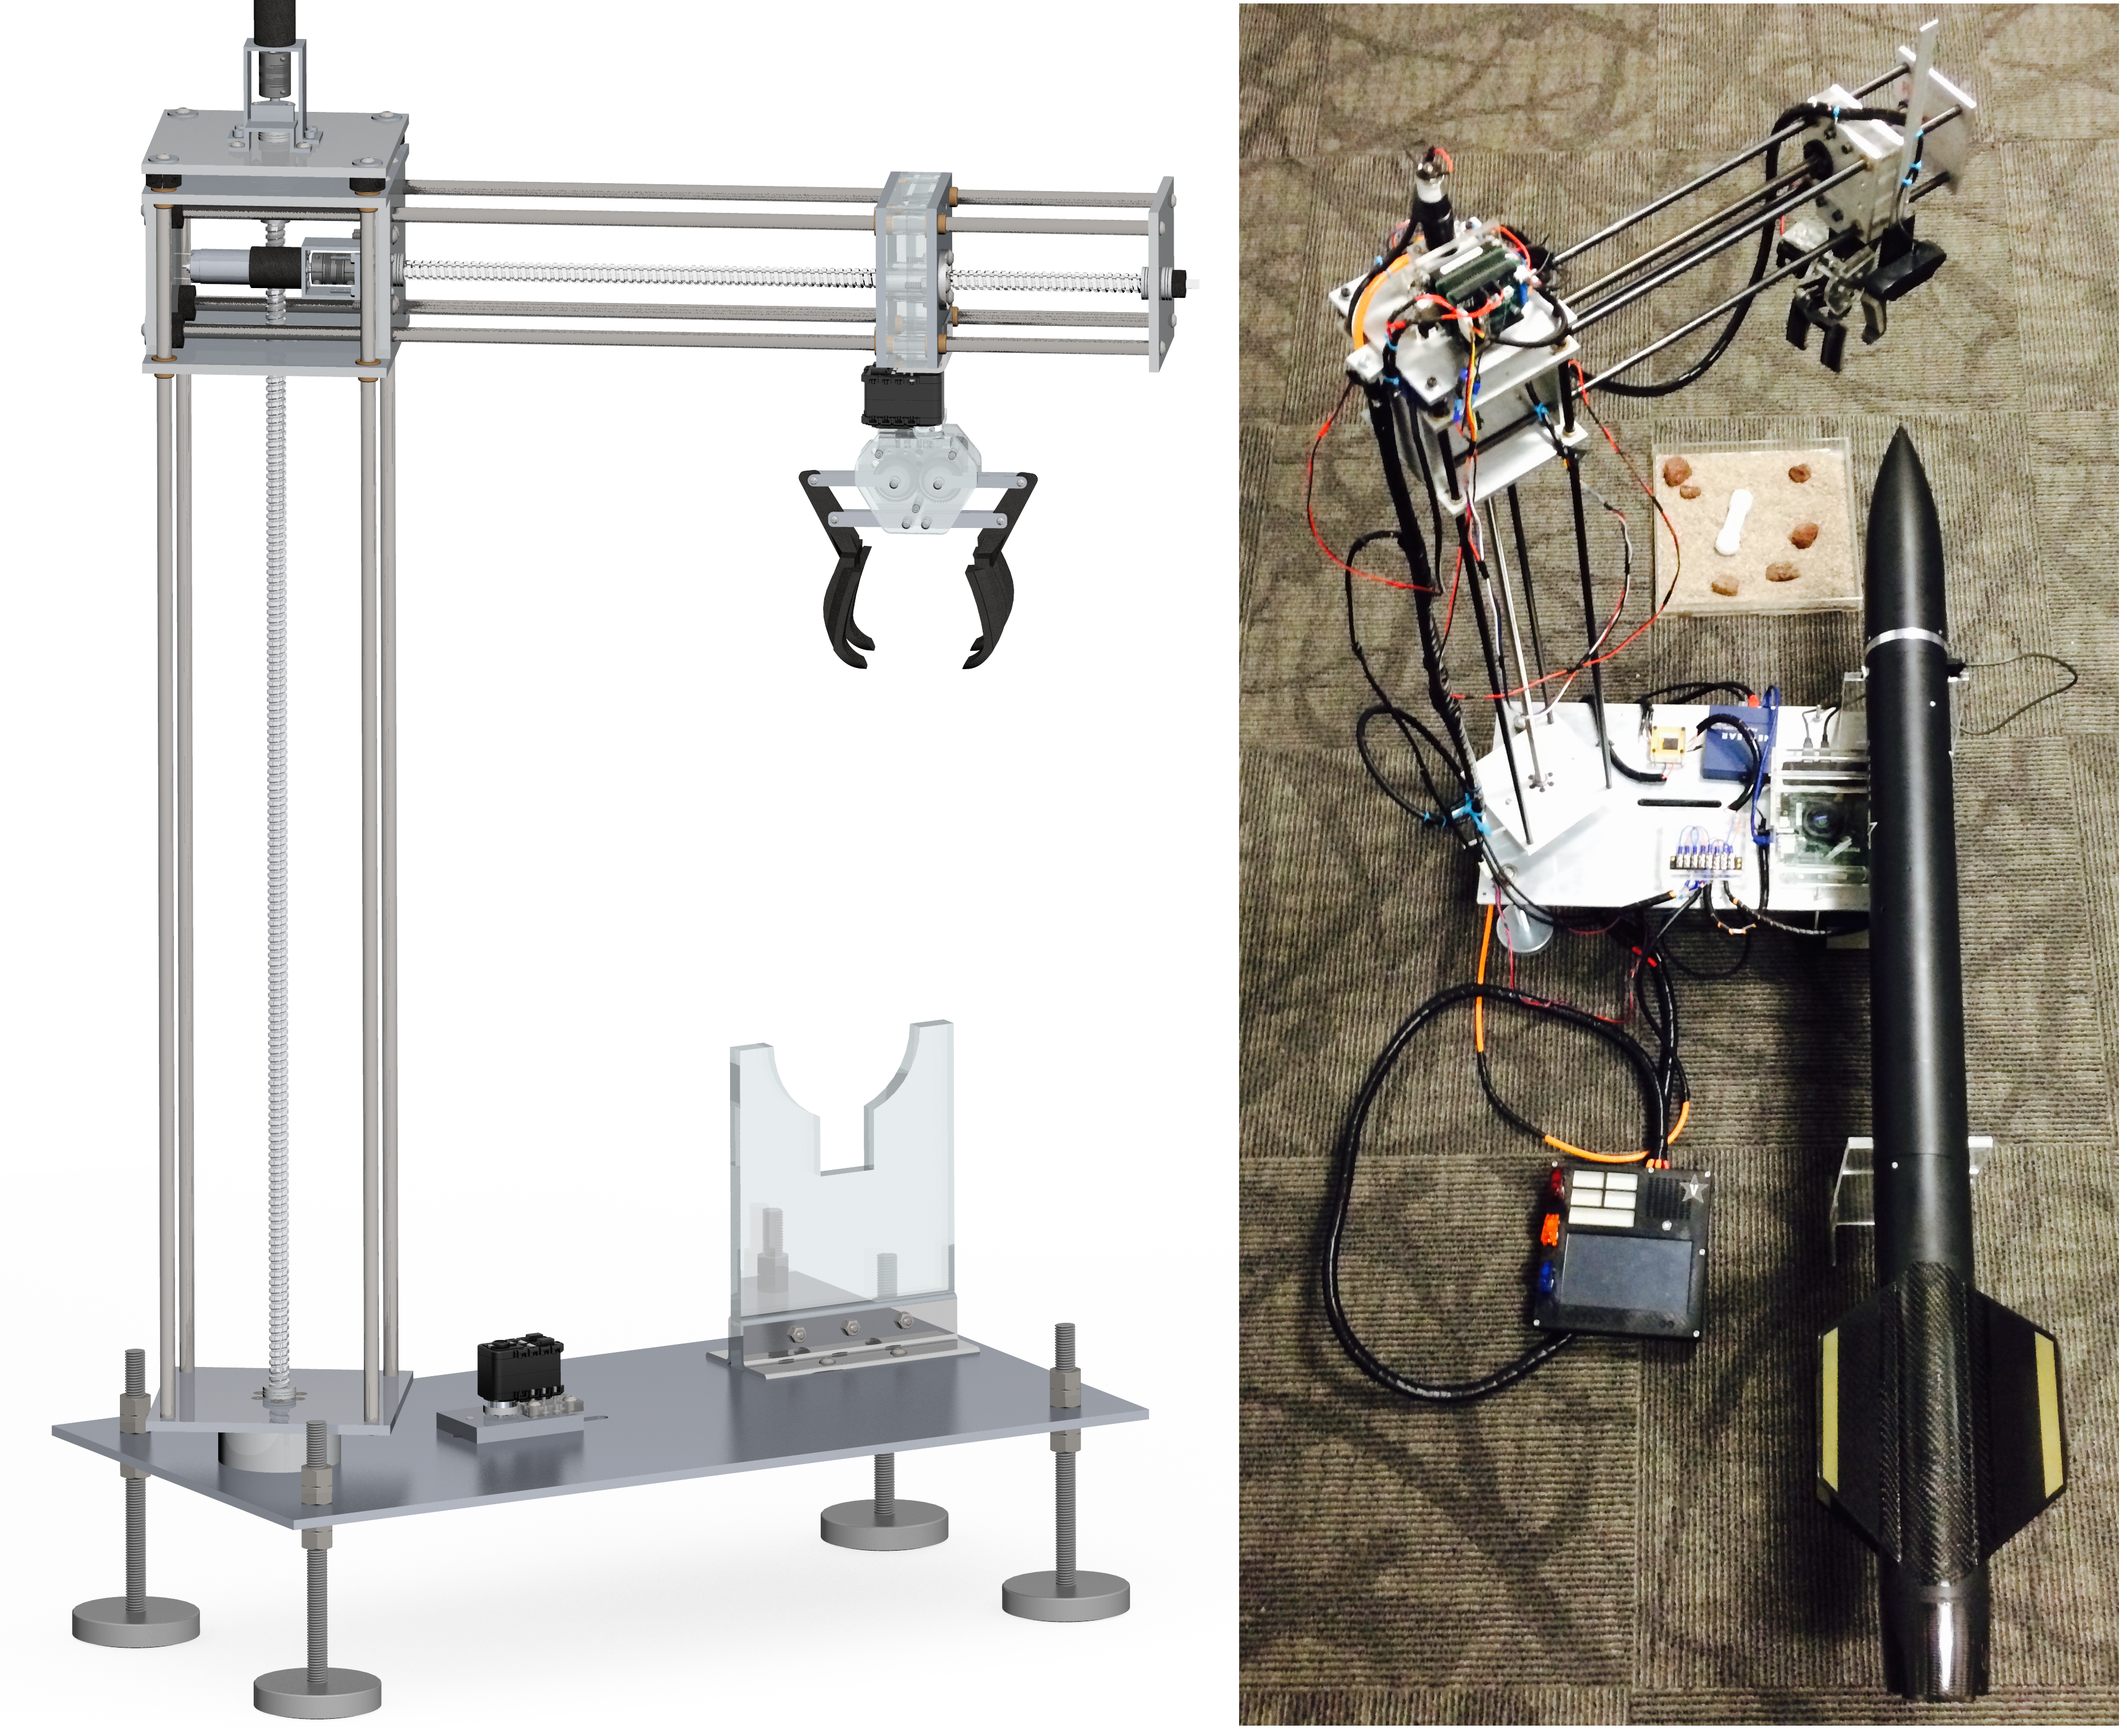
\includegraphics[width=\textwidth]{./Figures/AGSE_Render.png}
	\caption{AGSE and rocket used in the 2014-2015 NASA SLI
          competition.  The UIP is shown in the bottom left of the
          picture, the Motor Control Board is on the top of the arm of
          the AGSE, and the NVIDIA Jetson is under the rocket.}
	\label{fig:competition_AGSE}
\end{figure}


%  This section may be divided by subheadings. It should provide a concise and precise description of the experimental results, their interpretation as well as the experimental conclusions that can be drawn. 

\section{Results}

\if 0 This section may be divided by subheadings. It should provide a
concise and precise description of the experimental results, their
interpretation as well as the experimental conclusions that can be
drawn.

%%%%%%%%%%%%%%%%%%%%%%%%%%%%%%%%%%%%%%%%%%
\subsection{Subsection}
\subsubsection{Subsubsection}

Bulleted lists look like this:
\begin{itemize}[leftmargin=*,labelsep=4mm]
\item First bullet
\item Second bullet
\item Third bullet
\end{itemize}

Numbered lists can be added as follows:
\begin{enumerate}[leftmargin=*,labelsep=3mm]
\item First item
\item Second item
\item Third item
\end{enumerate}

The text continues here.

\subsection{Figures, Tables and Schemes}

All figures and tables should be cited in the main text as Figure 1,
Table 1, etc.

\begin{figure}[H]
  \centering %\includegraphics[width=3cm]{./Figures/logo-mdpi}
  \caption{This is a figure, Schemes follow the same formatting. If
    there are multiple panels, they should be listed as: (\textbf{a})
    Description of what is contained in the first panel. (\textbf{b})
    Description of what is contained in the second panel. Figures
    should be placed in the main text near to the first time they are
    cited. A caption on a single line should be centered.}
\end{figure}   

\begin{table}[H]
  \caption{This is a table caption. Tables should be placed in the
    main text near to the first time they are cited.}  \small % Font
  size can be changed to match table content. Recommend 10 pt.
  \centering
  \begin{tabular}{ccc}
    \toprule \textbf{Title 1} & \textbf{Title 2} & \textbf{Title
      3}\\ \midrule entry 1 & data & data\\ entry 2 & data &
    data\\ \bottomrule
  \end{tabular}
\end{table}

\subsection{Formatting of Mathematical Components}

This is an example of an equation:

\begin{equation}
  \mathbb{S}
\end{equation}

%% If the documentclass option "submit" is chosen, please insert a blank line before and after any math environment (equation and eqnarray environments). This ensures correct linenumbering. The blank line should be removed when the documentclass option is changed to "accept" because the text following an equation should not be a new paragraph. 
Please punctuate equations as regular text. Theorem-type environments
(including propositions, lemmas, corollaries etc.) can be formatted as
follows:
%% Example of a theorem:
\begin{Theorem}
  Example text of a theorem.
\end{Theorem}
The text continues here. Proofs must be formatted as follows:

%% Example of a proof:
\begin{proof}[Proof of Theorem 1]
  Text of the proof. Note that the phrase `of Theorem 1' is optional
  if it is clear which theorem is being referred to.
\end{proof}
The text continues here.  \fi
%%%%%%%%%%%%%%%%%%%%%%%%%%%%%%%%%%%%%%%%%%

\subsection{Performance Assessment}

At the competition, the Vanderbilt AGSE was able to complete the
sample retrieval process in approximately $4.5$ minutes. The recovery
process, as shown in Figure \ref{fig:AGSE_Operation}, was successful,
with payload and rocket bay recognition occurring quickly and
efficiently. The AGSE was able to grasp the payload using only two of
its four padded end effector phalanges, and successfully deposited the
payload within the rocket bay. This operation received high marks from
the NASA officials and earned the competition's \emph{Autonomous
  Ground Support Equipment Award}.

\begin{figure}[t]
  \centering
  \includegraphics[width=0.75\linewidth]{Figures/AGSE_Operation.png}
  \caption{AGSE Calibration and Testing}
  \label{fig:AGSE_Operation}	
\end{figure}

System robustness was validated on the day of competition when a key
component failed and was able to be quickly replaced with a different
part with no detriment to system performance. The Dynamixel AX-12A
servo controlling the base rotational degree of freedom of the AGSE
suffered an irreparable failure of its gearbox and had to be removed
from the robot. A backup of the servo was not readily available, and a
different model servo by the same company had to be swapped in
instead.  This new model, a Dynamixel MX-28T, while having similar
performance as the old servo, had a different communication protocol
and mounting footprint, as well as a more complex control scheme.

The component-based nature of ROSMOD allowed quick modifications of
the business logic of the \emph{rotation\_controller} component to
update the system to use the new hardware.  The new control scheme was
quickly implemented and the control software was updated to account
for the new physical placement of the servo due to its different
mounting footprint. After these modifications were made, the AGSE was
able to perform at its optimal level during its part of the
competition.


% This section may be divided by subheadings. Authors should discuss
% the results and how they can be interpreted in perspective of
% previous studies and of the working hypotheses. The findings and
% their implications should be discussed in the broadest context
% possible. Future research directions may also be highlighted.

\section{Discussion}

% This section may be divided by subheadings. Authors should discuss
% the results and how they can be interpreted in perspective of
% previous studies and of the working hypotheses. The findings and
% their implications should be discussed in the broadest context
% possible. Future research directions may also be highlighted.

%%%%%%%%%%%%%%%%%%%%%%%%%%%%%%%%%%%%%%%%%%

The goal of ROSMOD is to be a model-driven, component-based rapid
development, deployment, and experimentation toool suite for
distributed CPS.  This goal has been the driving force since the
beginning of ROSMOD during the 2014-2015 NASA SLI competition with the
AGSE.  ROSMOD itself was developed alongside the AGSE and in concert
with it; as we added features to the modeling language, the user
interface, or the generation and deployment infrastructure, we
immediately tested them with the AGSE.  The focus on the development
was always model-driven engineering coupled with component-based
software design principles enabling an iterative development cycle for
both the AGSE and ROSMOD.  Because of the competition's deadlines, we
focused on developing the AGSE and ROSMOD through short cycles between
design, implement, test, iterate.  These deadlines helped focus the
core of ROSMOD's architecture towards one of rapid system design,
development, and deployment.

Through this development cycle, our team had to maintain a balance
between many (sometimes conflicting) design considerations:

\begin{itemize}
\item utilizing component-based design to parallelize the development
  effort into subunits among each member
\item evolution of the design in concert with evolution of the
  implementation: must prototype and test quickly, but the
  implementation should be usable for the next phase of the design.
\item track and plan for materials lead-time, and testing/integration time
\item tool support, i.e. mechanical facilities and software
  development/testing support
\item expertise required for each component/subsystem design,
  development, and testing
\item importance of meaningful feedback especially with respect to
  errors and failures in software/hardware.
\end{itemize}

As in any software or hardware development, bugs and failures were
encountered in the development of both the AGSE hardware and software.
However, the use of the ROSMOD infrastructure allowed the causes of
those issues to be narrowed down and more quickly resolved.  For
example, the logging and tracing framework of ROSMOD enabled the
resolution of issues stemming from slow processor speed leading to
long execution times.  By using the logging and plotting features of
ROSMOD to trace the execution time of the component operations in the
AGSE software, we were able to determine that the NVIDIA Jetson was
running sub-optimally, and confirmed that the CPU frequency governor
was configured by default to dramatically throttle the main ARM cores
of the processor.  Furthermore, we were able to use the logging
framework to show that for some of the client-server connections in
the AGSE that were configured to be persistent connections, the
connection would drop immediately after being established.  After
determining this from the trace logs, we reconfigured those
client-server connections to no longer be persistent so they would
reconnect when required.

One of the main benefits from this timing and performance logging
infrastructure was the ability to validate the periodicity of timer
interactions in the AGSE.  By running the AGSE software and tracking
how long each operation takes, we were able to determine that the
original configuration of the AGSE timers was too frequent and needed
to be reduced by a factor of four.  By specifying deadlines on the all
the operations (esp. timer, server, and subscriber) we were able to
determine the bottlenecks in the system and figure out what parts of
the system had deadline violations (i.e. their execution times
exceeded their periodicity) and re-adjust the timers accordingly.

Figure \ref{fig:ExecPlot-armTimer} shows the execution time plot of the \emph{armTimer\_operation} in the high-level controller component. For sake of brevity, we avoid showing all the operational plots. In the context of Figure \ref{fig:AGSE}, this timer operation represents the execution of the high-level control state machine. The high-level controller communicates with multiple components over its life-span orchestrating various parts of the overall state machine e.g. initialization, sample detection, payload bay detection etc. Choosing an optimal period for this timer is necessary for many reasons. Firstly, the ROSMOD component operation scheduling is a non-preemptive one i.e. an operation must run to completion before the next request is serviced from the component operation queue. This means that if the timer operation does not complete before its period, the number of waiting requests in component queue start to monotonically rise. This hurts the system as a whole since subsequent requests take longer to complete and the high-level control breaks down. Secondly, inside the timer operation, the controller requires the services of both the motor control and the imaging components, often times via synchronous blocking interactions. This is the second cause of a potential problem as the blocking times are non-deterministic and dependent on the execution state of other embedded boards. For this reason, the AGSE software was deployed and experimented with to identify the optimal period where the response times are manageable. As shown in Figure \ref{fig:ExecPlot-armTimer}, the high-level controller has two set of spikes in execution time. The first set (between 100 and 150 seconds into the experiment), as confirmed by Figure \ref{fig:ExecPlot-sample-Bay-DetectionStateFromImageServer} corresponds to sample detection. The second set of spikes, between 200 and 250 seconds, is the payload bay detection. These plots quickly present the performance of the high-level controller and the worst-case response times during periodic image processing. 

\begin{figure}[t]
	\centering
	\includegraphics[width=\linewidth]{Figures/ExecPlot-armTimer.png}
	\caption{High-level Timer Execution}
	\label{fig:ExecPlot-armTimer}	
\end{figure}

\begin{figure}[t]
	\centering
	\includegraphics[width=\linewidth]{Figures/ExecPlot-sample-Bay-DetectionStateFromImageServer.png}
	\caption{Sample and Payload bay Detectors Execution}
	\label{fig:ExecPlot-sample-Bay-DetectionStateFromImageServer}	
\end{figure}

Figure \ref{fig:ExecPlot-sample-Bay-DetectionStateFromImageServer} presents the performance of the \emph{GetSampleState\_Server} and the \emph{GetPayloadState\_Server} in Figure \ref{fig:AGSE}. These servers are periodically invoked by the high-level controller during its operation, first during sample detection and then during payload bay detection. Each of these servers, on demand, are required to obtain the current camera feed from the Camera component, perform image processing, and return the results to the high-level controller. Thus, the interaction and data flow path is as follows: During sample detection, the high-level controller is periodically triggered to ask the Image Processor component to provide a new result. The Image Processor, in turn, queries the Camera component for a feed update. The Camera \emph{ImageServer}, as shown in Figure \ref{fig:ExecPlot-captureImage} responds to the Image Processor component with a new feed. This image server is also responding to the userDisplay component that receives the camera feed to display to the user. 

\begin{figure}[t]
	\centering
	\includegraphics[width=\linewidth]{Figures/ExecPlot-captureImage.png}
	\caption{Camera Feed Reponse Times}
	\label{fig:ExecPlot-captureImage}	
\end{figure}

Wwe were able to use the ROSMOD deployment infrastructure to
quickly run separate experiments on the BeagleBone Blacks (single core
embedded computers), testing the performance impact of running our
motor control components in separate processes or as separate threads
in the same process.  By simply changing the deployment model and
re-running the same code we were able to get ROSMOD timing and
performance logs from the experiments to show the extra overhead of
process-level context switching on the single-core BeagleBone Black.

The use of ROSMOD's performance, timing, and trace logging (coupled
with the plotting utilities for those logs) enabled us to easily
visually verify the behavior and performance of the AGSE software or
spot anomalies when they occurred.  Furthermore, the use of
code-generation and automated build and deployment infrastructure
meant that far less code had to be inspected for errors when a
software or logical error cropped up, and the developers did not have
to spend time configuring or debugging the build and deployment
systems.  Finally, the use of a graphical modeling tool for specifying
the entire AGSE project from software to hardware to deployment
enabled faster training and communications between team members as
well as visual inspection of the software configuration, for instance
ensuring that all required components can respond to the user's
control inputs or verifying the other interaction patterns and
triggering operations for each component.

The rapid prototyping facilitated by ROSMOD and the ROS infrastructure
enabled the development of an overall \emph{smarter} robot. The
software requirements for autonomy were matched by the ROSMOD code
generators such that developers had to spend little time setting up
the build system and interaction patterns. The speed of development
was drastically improved and the \emph{business logic} code, i.e. the
core of the implementation of the system behavior, could be made more
robust in spite of the evolution of and inclusion of more autonomy.

\iffalse
Mention that the hardware for the robot was designed and developed
primarily by 2-4 people (dexter can decide) and the electronics and
software for the robot was designed and developed by 2 people, at the
same time that the ROSMOD toolsuite was developed.

Mention the pitfalls we encountered (w.r.t. using the logger to
realize the speed of the jetson, the client-server failure when
turning on persistent connections, the mechanical hardware, the
electrical hardware, lead time and shipping, model translation and
update from V0.3 to V1.0, etc.)
\fi

\section{Materials and Methods}
% This section should be divided by subheadings. Materials and Methods
% should be described with sufficient details to allow others to
% replicate and build on published results. Please note that publication
% of your manuscript implicates that you must make all materials, data,
% and protocols associated with the publication available to
% readers. Please disclose at the submission stage any restrictions on
% the availability of materials or information. New methods and
% protocols should be described in detail while well-established methods
% can be briefly described and appropriately cited.
%
% Research manuscripts reporting large datasets that are deposited in a
% publicly available database should specify where the data have been
% deposited and provide the relevant accession numbers. If the accession
% numbers have not yet been obtained at the time of submission, please
% state that they will be provided during review. They must be provided
% prior to publication.

This section covers the materials and methods for ROSMOD and the AGSE,
both what was used in the competition (2014-2015) as well as the
current state of each.

\subsection{Competition AGSE}

The version of the AGSE software and hardware designs that were used
in the 2014-2015 NASA SLI competition can be found open-sourced
online\cite{AGSE2015}. The current version of the AGSE code and
hardware designs has been moved and can be found in the Vanderbilt
Aerospace Design Lab's AGSE repository\cite{AGSE}.

\subsubsection{Kinematics}
%describe the joint structure of the robot, detail the coordinate system, etc.

The AGSE is a 4-DOF robot utilizing a revolute base joint to rotate
the robot body, two prismatic joints to move vertically and
horizontally, and a final revolute joint providing an orienting wrist
for the end effector. A wireframe and workspace rendering of the AGSE
can be seen in Figure \ref{fig:Render}.


\begin{figure}[h]
	\centering
        \includegraphics[width=\textwidth]{./Figures/AGSE_Mechanical_Design_Figure.png}
	\caption{AGSE Mechanical Design}
	\label{fig:Render}
\end{figure}

%description of coordinate system
By design, the single revolute and two prismatic joints of the AGSE
provide the basis for a cylindrical coordinate system and workspace,
reducing the implementation of both forward and reverse kinematics to
a trivial exercise of mapping joint position to the corresponding
coordinate in the workspace.

$$
\begin{bmatrix}
	\boldsymbol{\theta}_{workspace}\\\mathbf{r}_{workspace}\\\mathbf{z}_{workspace}
\end{bmatrix}=
\begin{bmatrix}
	\boldsymbol{\theta}_{rev}\\\mathbf{r}_{pris}\\\mathbf{z}_{pris}
\end{bmatrix}
$$
%?equations of end-effector position based on joint posiiton?

\subsubsection{Structure}
%describe the physical structure of the base, each joint starting at the base, mounting hardware for electronics

The AGSE base is comprised of a machined sheet of aluminum upon which
leveling legs are mounted to easily account for uneven surfaces.
Protruding from the base is the revolute joint, a machined spindle
centered within ball bearing cup. Extending upwards along this
rotational axis is the vertial join, a lead screw and guide rod
assembly driving an aluminum carriage. A similar lead screw-carriage
assembly extends from the side of the vertical carriage to provide
motion within the horizontal plane. A mounting point for both the
gripper and camera hangs from this horizontal carriage.

Underneath the base is a platform for mounting batteries, power
regulation and protection circuitry, and on-board computer systems.  At
the top of the vertical assembly is a mounting point for the actuator
control electronics.


\subsubsection{Actuation and Sensing}
%detail the actuators used for each joint and all sensors utilized

A Dynamixel MX-28T servo is mounted to the revolute joint's spindle to
provide rotational movement. Two additional Dynamixel AX-12 servos are used
to orient and actuate the gripper. The two lead screw assemblies are
driven using 12 V Faulhaber motors mounted directly to the lead
screws.

The AGSE guides the end effector motion using the limit switch-encoder
combo on its linear actuators, the built in positional feedback from
the servo motors, and the optical feedback provided by a camera
mounted above the end effector (allowing the AGSE to recognize objects
within the reachable area underneath the gripper phalanges).  Limit
switches are mounted at the minimum and maximum of each lead screw
assembly's range of movement, providing hard stops to motor actuation.
Quadrature encoders are then used within this range of motion to
monitor the position of the vertical and horizontal carriages. The
Dynamixel servos controlling the revolute joint and gripper provide
position and speed feedback, as well as PID tuning to allow for quick
and responsive control.

\subsubsection{Power System}
%What powers it: Originally 2 12v batteries, now using power supply
%On/Off with relay
%Power Protection: Originally none, now have a fuse board
%

The power from the AGSE comes from two 12V 12Ah lead-acid batteries in
series, which provide input power to a 12V power regulator.  The 12V
output from the power regulator passes through a relay which is
controlled using a key-switch on the User Interface Panel (UIP).  From
the relay the 12V runs in parallel to the NVIDIA Jetson TK1, the Motor
Control Cape on the Motor Control BeagleBoneBlack, the User Interface
Panel power control cape (a stripped down version of the Motor Control
Cape with the H-Bridges and other motor related electronics not
populated), and finally to the ethernet switch which provides a
closed, hard-wired LAN for communications between the boards.

On the Motor Control Board, the 12V input drives 1) the cape's 5V
regulator which provides power to the BeagleBone Black and the
encoders, 2) the 12V Dynamixel servo motors, and 3) the H-Bridges for
the two 12V linear actuators.

On the UIP, the 12V simply powers the 5V regulator which provides
power to the BeagleBone Black, the touchscreen LCD, and the display
LEDs.

\subsubsection{Control}
%Touch on these topics: Low-Level Motor Control, High-Level control  (Introduce image processing and path planning), feedback processing

The payload bay and nose section of the rocket rests on the base of
the AGSE. This payload bay is motor-controlled by the high-level
controller. When the AGSE starts up, the payload bay's on-board Arduino motor controller is
commanded to open the nosecone. Once open, the AGSE performs an initialization
routine. This routine includes movement of the vertical and radial
actuators to a safe height and a retracted state. Then, the AGSE
rotates on its base to a servo angle of zero degrees. Once this
routine is complete, the robots begins searching for the sample. The
camera used for this purpose is a 1920x1080 wide resolution feed; one
that enables the robot to sweep wider distances when searching for the
sample and increases the step size of the search i.e. the search steps
up by 20 degree increments while searching for the sample.

\begin{figure}[h]
	\centering
	\includegraphics[width=0.75\textwidth]{Figures/Sample_Image_Processing_2.png}
	\caption{AGSE Sample Detection - Periodic Image Processing}
	\label{fig:Sample_Image_Processing_2}
\end{figure}

Periodic sample detection performed by the AGSE uses OpenCV-based
image processing algorithms to identify and track the sample in
real-time. An Image Processor component periodically fetches the
latest feed from the mounted camera and performs a series of filtering
tasks. Each \emph{RGB} (Red-green-blue) image frame is converted to
both \emph{HSV} (Hue-Saturation-Value) and \emph{Grayscale} image
frames. After applying thresholds, filters, erosion and dilation
methods, the target sample is extracted from the webcam feed. Once the
target sample is detected, as shown in Figure
\ref{fig:Sample_Image_Processing_2}, we draw contours around the
object and identify its relative position and orientation.

Once the sample is detected, the AGSE records the position and
orientation of this sample and begins searching for the payload
bay. The payload bay is detected using marker detection methods. Coded
markers are stuck on the payload bay to detect the angle at which the
sample needs to be dropped into the bay. As shown in Figure
\ref{fig:Payloadbay_Detection}, by processing the input camera feed,
the two markers on the bay are detected and the angle of drop is
calculated.

\begin{figure}[h]
	\centering
	\includegraphics[width=0.75\textwidth]{Figures/Payloadbay_Detection.png}
	\caption{AGSE Payload Bay Detection}
	\label{fig:Payloadbay_Detection}
\end{figure}

Once the sample and payload bay are fully detected, the AGSE performs
a simple pickup-drop transition where it rotates to the position of
the sample, grabs the sample, rotates to the position of the payload
bay and drops the sample in the bay. The arm control logic also sends
a \emph{"Close Payload Bay"} command that actuates the payload motor
and closes the nosecone, effectively completing the sample retrieval
process.

\subsubsection{Communication}
%How do the components communicate? Servos daisychained and identified by device ID and controled via modified dynamixel library, BBB, Jetson, and UIP connected to network with static IPs, etc.

The AGSE communicates between its various subsystems using a few
different protocols.  At the high level, the different control boards
of the AGSE communicate using ROS over a wired ethernet LAN.  On the
motor control board, the servo motors are directly connected to a 3.3V
serial port on the GPIO pins of the BeagleBone Black.  Because the
servo motors communicate at 5V using a 1-wire communications line, the
communications transmitted to the servos from the BeagleBone Black
passes through a buffer implemented with NPN transistors.  Because the
servos can be daisy-chained, only one connection is made to the Motor
Control Cape and each servo is connected in series through the
previous servo.  This daisy-chaining greatly simplifies the wire
routing and increases the modularity and maintainability of the AGSE
motor hardware.  Finally, the NVIDIA Jetson communicates to the
Payload Bay Arduino to open and close through its own USB port acting
as a virtual serial port.  This serial connection is implemented as a
quick-disconnect USB cable connected to a port on the surface of the
rocket.

\subsection{AGSE Changes Since the Competition}

Post competition, minor mechanical and electrical improvements were made to the AGSE.  A new mounting bracket was machined to replace the temporary mounting of the Dynamixel MX-28T that occurred the day of the competition. A new undercarriage made of extruded 20mmx20mm aluminum was fabricated to house the on-board power circuitry and embedded systems.  Additionally, new power protection circuitry was made in the form of fuse boards and a dedicated emergency stop button in lieu of the key switch in the UIP.

\subsection{Competition ROSMOD}

ROSMOD exists as two separate code-bases: 1) the ROSMOD component
model implementation, which enables the configuration of the component
operation queue to support different scheduling schemes and
priorities/deadlines for operations, and 2) the ROSMOD graphical
modeling, generation, and deployment tool suite.  These two code-bases
are referred to as ROSMOD-COM and ROSMOD-GUI, respectively.  All
ROSMOD related code (old and new) can be found open-sourced online in
the ROSMOD Github organization\cite{ROSMOD_ORG}.

ROSMOD-COM is a package which extends the functionality of the
\emph{ROS Callback Queue} into which timer, subscriber and service
operations are placed.  To enable the addition of scheduling,
priority, and deadline attributes to operations in the queue, all the
relevant objects were modified, e.g. Timer, Subscriber, etc.
Additionally, the queue was extended to support priority insertion of
operations based on their deadline (EDF scheduling) and priority
(PFIFO).  By using the relevant classes and methods from ROSMOD-COM,
ROSMOD components can ensure the proper scheduling of their
operations.

The version of ROSMOD that was used in the competition can also be
found open-sourced online\cite{ROSMOD}, as the \emph{v0.3-beta}
release.  Note that the version of the ROSMOD-GUI that was used is
under the \emph{gui} folder and is a Python-based program for which
the relevant dependencies must be installed following the
\emph{README}.  This is one of the primary problems with this version. Firstly, ROSMOD requires Linux and the Python programming language and a long list of dependencies. Also, this version, as used in the competition was primarily used for code generation and compilation. The deployment framework had several shortcomings, primarily due to the metamodeling language at the time. Many of these shortcomings have now been addressed e.g. the concept of an experiment, a much improved network model etc. 

\subsection{ROSMOD Changes Since the Competition}
The current version of ROSMOD is split into two
separate repositories under the ROSMOD organization: the new version
of the GUI\cite{ROSMOD_WEBGME}, and the current version of
ROSMOD-COM\cite{ROSMOD}.

ROSMOD-COM has been updated to be a standalone ROS package so that it
no longer has to be compiled inside ROS' source tree.  Upon installing
ROSMOD-COM, the scheduling schemes and associated configuration and
classes become available for use in all packages.

ROSMOD-GUI has been transformed into a more fully integrated
development environment which is now platform independent as it runs
within the browser.  The server runs within a Linux environment and
can be locally deployed on a laptop or virtual machine, or on a real
server.  The change to this new infrastructure was enabled by the
switch to using WebGME\cite{maroti2014next} as the backend for the modeling and
server execution.  This change also enables collaborative
simulataneous model creation and editing between multiple users, with
built-in git-sytle versioning, branching, and merging.

Despite the increase in backend complexity and number of features of
ROSMOD, the use of ROSMOD and the installation of the backend has
become far simpler and completely automated by widely-used packaging
tools.  The repository has installation instructions and users guides.

%\section{Conclusions}

This section is not mandatory, but can be added to the manuscript if the discussion is unusually long or complex.

%%%%%%%%%%%%%%%%%%%%%%%%%%%%%%%%%%%%%%%%%%

\vspace{6pt} 

%%%%%%%%%%%%%%%%%%%%%%%%%%%%%%%%%%%%%%%%%%
%% optional
%\supplementary{The following are available online at www.mdpi.com/link, Figure S1: title, Table S1: title, Video S1: title.}

%%%%%%%%%%%%%%%%%%%%%%%%%%%%%%%%%%%%%%%%%%
\acknowledgments{This work was supported by DARPA under contract NNA11AB14C and USAF/AFRL under Cooperative Agreement FA8750-13-2-0050, and by the National Science Foundation (CNS-1035655). The activities of the 2014-15 Vanderbilt Aerospace Club were sponsored by the Department of Mechanical Engineering and the Boeing Corporation. Any opinions, findings, and conclusions or recommendations expressed in this material are those of the author(s) and do not necessarily reflect the views of DARPA, USAF/AFRL, NSF, or the Boeing Corporation. Lastly, the authors would also like to thank the following undergraduate students on the AGSE design team for their invaluable work: Connor Caldwell, Frederick Folz, Alex Goodman, Christopher Lyne, Jacob Moore and Cameron Ridgewell.}

%%%%%%%%%%%%%%%%%%%%%%%%%%%%%%%%%%%%%%%%%%

\authorcontributions{Gabor Karsai conceived and designed the ROSMOD component model. Pranav Srinivas Kumar and William Emfinger were the primary software developers for the ROSMOD toolsuite, the ROSMOD component model, and the AGSE control software. Amrutur Anilkumar and Benjamin Gasser designed the AGSE robot and lead the Vanderbilt Aerospace Design Laboratory. Dexter Watkins, and Benjamin machined and constructed the AGSE robot. William Emfinger performed the AGSE execution time experiments. Pranav Srinivas Kumar analyzed the data and generated execution plots. Pranav Srinivas Kumar, William Emfinger and Dexter Watkins wrote the paper.}

%%%%%%%%%%%%%%%%%%%%%%%%%%%%%%%%%%%%%%%%%%
\conflictofinterests{The authors declare no conflict of interest. The founding sponsors had no role in the design of the study; in the collection, analyses, or interpretation of data; in the writing of the manuscript, and in the decision to publish the results.} 

%%%%%%%%%%%%%%%%%%%%%%%%%%%%%%%%%%%%%%%%%%
%% optional
\abbreviations{The following abbreviations are used in this manuscript:\\
	
	\noindent AGSE: Autonomous Ground Support Equipment\\
	ARM: Advanced RISC Machines\\
	BBB: Beaglebone Black\\
	CNC: Computer Numerical Control\\
	CPS: Cyber-Physical System\\
	CPU: Central Processing Unit\\
	CUDA: Compute Unified Device Architecture\\
	CV: Computer Vision\\
	DARPA: Defense Advanced Research Projects Agency\\
	DOF: Degrees of Freedom\\
	EDF: Earliest Deadline First\\
	FIFO: First-In First-Out\\
	GPIO: General Purpose Input/Output\\
	HSV: Hue-Saturation-Value\\
	IP: Internet Protocol\\
	LAN: Local Area Network\\
	LCD: Liquid Crystal Display\\
	LED: Light Emitting Diode\\
	MAV: Mars Ascent Vehicle\\
	NASA: National Aeronautics and Space Administration\\
	PFIFO: Priority First-In First-Out\\
	PID: Proportional-Integral-Derivative\\
	QEP: Quadrature Encoded Pulses\\
	RGB: Red-Green-Blue\\
	RMI: Remote Method Invocation\\
	RML: ROSMOD Modeling Language\\
	ROS: Robot Operating System\\
	SFIO: Special Function Input/Output\\
	SSH: Secure Socket Shell\\
	SLI: Student Launch Initiative\\
	UAV: Unmanned Aerial Vehicle\\
	URL: Uniform Resource Identifier\\
	UUV: Unmanned Underwater Vehicle\\
	UIP: User Interface Panel\\
	USB: Universal Serial Bus\\
	XML: Extensible Markup Language\\}

%%%%%%%%%%%%%%%%%%%%%%%%%%%%%%%%%%%%%%%%%%
%% optional
%\appendix
%\section{}
%The appendix is an optional section that can contain details and data supplemental to the main text. For example, explanations of experimental details that would disrupt the flow of the main text, but nonetheless remain crucial to understanding and reproducing the research shown; figures of replicates for experiments of which representative data is shown in the main text can be added here if brief, or as Supplementary data. Mathemtaical proofs of results not central to the paper can be added as an appendix.

%\section{}
%All appendix sections must be cited in the main text. In the appendixes, Figures, Tables, etc. should be labeled starting with `A', e.g., Figure A1, Figure A2, etc. 

%%%%%%%%%%%%%%%%%%%%%%%%%%%%%%%%%%%%%%%%%%
\bibliographystyle{mdpi}

%=====================================
% References, variant A: internal bibliography
%=====================================
\renewcommand\bibname{References}
\bibliography{JoE2016-Bibliography}
%\begin{thebibliography}{999}
% Reference 1
%\bibitem{ref-journal}
%Lastname, F.; Author, T. The title of the cited article. {\em Journal Abbreviation} {\bf 2008}, {\em 10}, 142-149.
% Reference 2
%\bibitem{ref-book}
%Lastname, F.F.; Author, T. The title of the cited contribution. In {\em The Book Title}; Editor, F., Meditor, A., Eds.; Publishing House: City, Country, 2007; pp. 32-58.
%\end{thebibliography}

%=====================================
% References, variant B: external bibliography
%=====================================
%\bibliography{your_external_BibTeX_file}

%%%%%%%%%%%%%%%%%%%%%%%%%%%%%%%%%%%%%%%%%%
%% optional
%\sampleavailability{Samples of the compounds ...... are available from the authors.}

%%%%%%%%%%%%%%%%%%%%%%%%%%%%%%%%%%%%%%%%%%
\end{document}

